\documentclass{article}
\usepackage[utf8]{inputenc}
\usepackage[margin = 0.8in]{geometry}
\usepackage{graphicx}
\usepackage{amsmath, amssymb}
\usepackage{subcaption}
\usepackage{multirow}
\usepackage{mathtools}
\usepackage{float}


\title{RBE550 - Transmission RRT Assignment}
\author{Keith Chester}
\date{Due date: April 25 2022}

\begin{document}
\maketitle

\section*{Introduction}

In this assignment, we aim to demonstrate RRT planning in a 3d dimensional environment by utilizing the algorithm to plan a collision free removal of the primary shaft out of a SM-465 transmission gearbox. The tight interior of the gear box makes for a difficult multidimensional planning problem that will require six dimensions of planning (x, y, z, as well as roll, pitch, and yaw).

\section*{Simulation of Environment}
For this project, we first modeled both the primary shaft (the top shaft we will be moving through 3D space out of the transmission), the fixed shaft (the bottom shaft), and the walls of the transmission. For clarity, we do not draw the side walls of the transmission.

To accomplish this, we utilized MATLAB's rigid body trees and collision geometries to create a close simulacrum of our transmission based on provided STL files. The image below shows our results:

\begin{figure}[H]
    \centering
    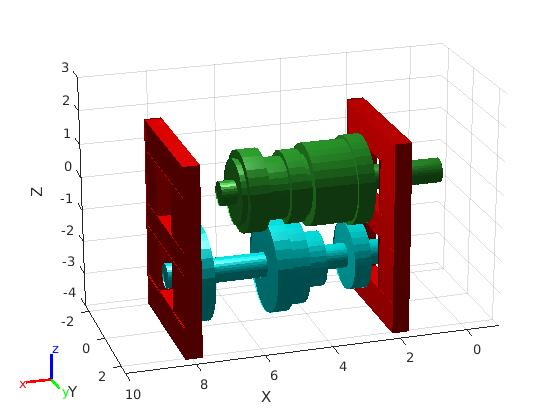
\includegraphics[width = 0.75\textwidth]{img/start.jpg}
    \caption{SM-465 Transmission}
    \label{fig:start}
\end{figure}

\section*{RRT Path Planning Approach}

To generate an RRT path, we define both the start position and the goal. We treat each degree of freedom - 3 translations and 3 rotations - as a dimension. We produce random points within the spectrum of these 6 dimensions (though, admittingly, we severely limit two axis of rotations as they are not strictly needed for this problem). Each time we generate a node, we find the closest node attached to our tree (beginning with our root, the start node). We create a movement in each dimension towards the random node some small iterative step each time. This produces a tree with significant branching into exploration.

To speed up the process of finding a path to our goal, we randomly select the goal node instead of a random node. This encourages growth in the tree's branches towards the goal, and not just out to random space.

Once we generate these new poses within for our tree, we perform a collision check before attaching it. If the collision checker finds that the primary shaft would collide with the fixed shaft or the walls of the transmission, we ignore the generated point and move on.

Once the a branch node is within an acceptable distance to the goal, we connect them. Each node, upon generation, is assigned a reference back to its parents - as such, we can traverse these references to create the entire path from the goal to the start node - our path!

\section*{Resuls}

\begin{figure}[H]
    \centering
    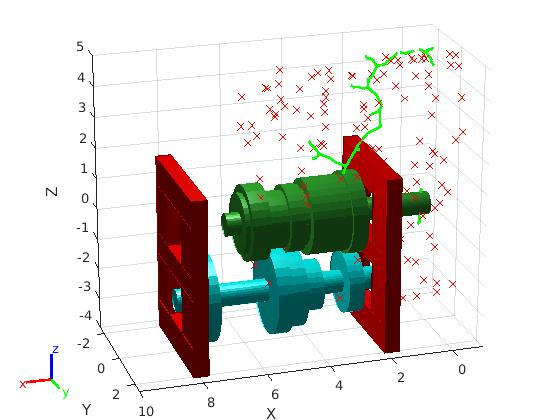
\includegraphics[width = 0.75\textwidth]{img/plan.jpg}
    \caption{SM-465 Transmission}
    \label{fig:path}
\end{figure}

Here we see random nodes placed as red X's in our workspace. The tree is represented as a series of green lines. Note that we can only represent 3 dimensions here - X, Y, and Z, though each node and tree represented a six dimensional value. We see that the tree has random branching, but ultimately favored going towards our desired goal position.

\begin{figure}[H]
    \centering
    \begin{subfigure}{0.4\textwidth}
        \centering
        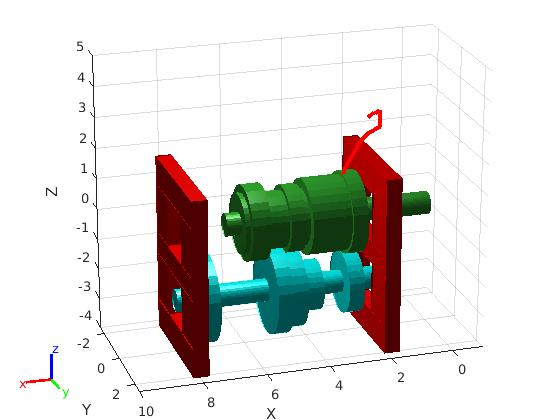
\includegraphics[width = \textwidth]{img/pose_1.jpg}
    \end{subfigure}
    \begin{subfigure}{0.4\textwidth}
        \centering
        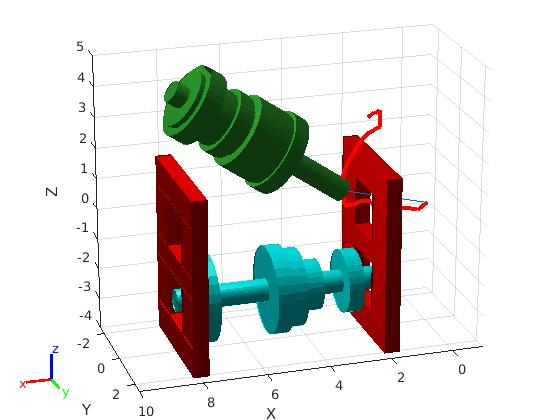
\includegraphics[width = \textwidth]{img/pose_2.jpg}
    \end{subfigure}
    \begin{subfigure}{0.4\textwidth}
        \centering
        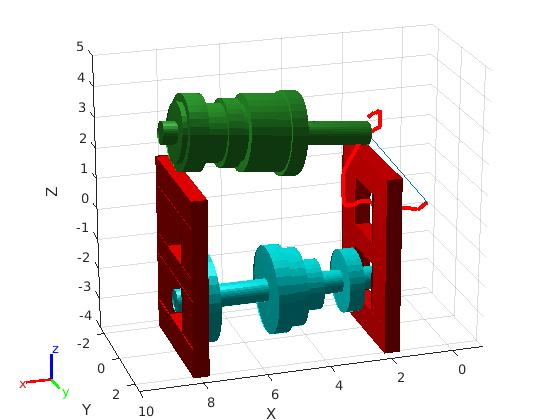
\includegraphics[width = \textwidth]{img/pose_3.jpg}
    \end{subfigure}
    \begin{subfigure}{0.4\textwidth}
        \centering
        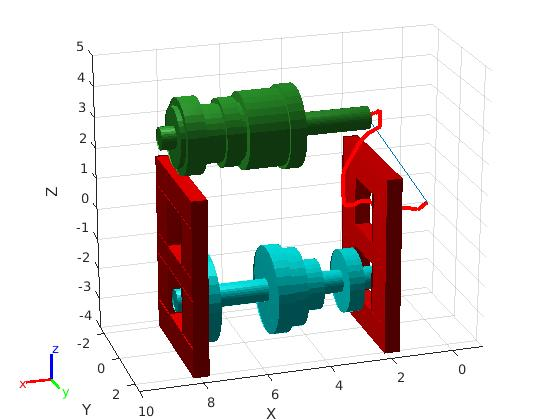
\includegraphics[width = \textwidth]{img/pose_4.jpg}
    \end{subfigure}
    \caption{The planned path in action}
    \label{fig:path-poses}
\end{figure}

In the above figure, we see the start and finally end poisition of our drive shaft, fully removed from its transmission. We also see the intermediate stages that the plan generated - properly rotating the shaft as well as moving it to find a way to move it out with contact.

\section*{Observations and Improvements}

Since RRT is a probabilistic algorithm, we did not find necessarily the smoothest or most optimal routes out. Several attempts running this algorithm created routes that, while successfull, resulted in large oscillations in the primary shaft that was not strictly necessary. This author does note, however, that RRT certainly took very few iterations to rapidly produce results, however. It seems that RRT is likely good for chaotic environments where exploration is more favored in a path planning algorithm.

We also implemented RRT over RRT* for its simplicity. RRT* would have created optimal routes for the branches discovered - also meaning that additional run time would likely produce more optimal and likely smoother paths.

Due to time constraints, we utilized a naive method of determining the closest node to our randomly selected points. We merely look at all existing nodes in our tree and calculate the distances for each, comparing to find the closest. This author realizes that this is a poor decision, and easily the single cause of latency in our path finder algorithm. It is clear that this part of the process can be optimized to produce far quicker results, such as utilizing KD-Trees or other memory structures for rapidly determining node proximity.

\section*{Conclusion}

This homework project's aim was to explore RRT as a path planning algorithm. To that end we developed a path planner for removing the primary shaft for a SM-465 transmission gearbox. Our path planner randomly explored space and eventually developed a tree of potential paths, with a singular branch leading the way for the starting pose of the shaft to be guided to our desired goal pose. We succeeded in this aim, and found firsthand the strengths and shortcomings of the algorithm.


\end{document}